\chapter{Revised Structure Models}

The results of the \ac{XPS} and \ac{NIXSW} measurements, that were discussed beforehand, have led to new insights regarding the adsorption height of \ac{QA} on the Ag(100) surface and especially the role of the hydrogen bonds in the $\beta$-phase. Based on these findings, revised structure models with the heights from the \ac{NIXSW} measurements for both the $\alpha$- and the $\beta$-phase are proposed in the following sections.

However, the lateral positions of the atoms in the structure models are still based on the structure models from the literature, which were discussed in \autoref{chap:literature} and based on \ac{LEED} and \ac{STM} measurements.\autocite{Humberg2020,Humberg2025} The covalent radii of the atoms are taken from reference \cite{Cordero2008}, while the van der Waals radii of the atoms are taken from reference \cite{Alvarez2013}. The structure models were created with ASE\autocite{HjorthLarsen2017}. As the adsorption heights of the H atoms could not be determined from the \ac{NIXSW} measurements, they were estimated based on the adsorption heights of the other atoms. Nevertheless, the H atoms are shown in the structure models for completeness, and their height is set to the same value as the height of the $\mathrm{C_{arom}}$ atoms.

\section{Structure model for the \texorpdfstring{$\alpha$}{alpha}-phase}

First, the structure model for the $\alpha$-phase of \ac{QA} on the Ag(100) surface is explained in more detail. The top view of the revised structure model is shown in \autoref{fig:qa_alpha_top_view}, while the long and short side views of the \ac{QA} molecule are shown in \autoref{fig:qa_alpha_long_side} and \autoref{fig:qa_alpha_short_side}, respectively.

\begin{figure}[htbp]
    \centering
    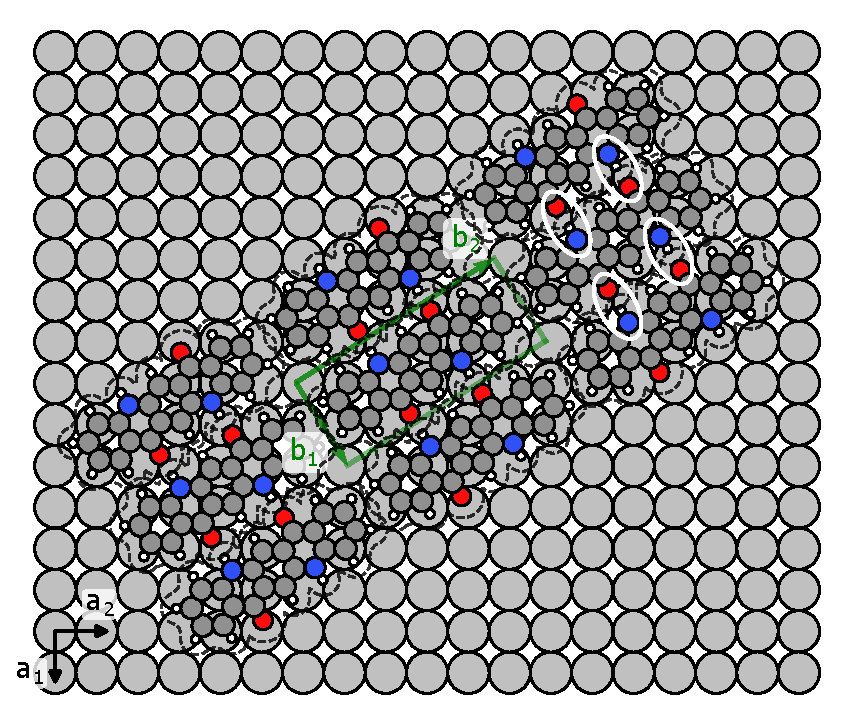
\includegraphics[width=\textwidth]{images/Models/qa_alpha-2_top-view_with_vdw-hbonds.pdf}
    \caption{Top view of the structure model for the $\alpha$-phase of \ac{QA} on the Ag(100) surface. The van der Waals radii of the atoms are shown as dashed grey lines, and the 4 hydrogen bonds of one \ac{QA} molecule to its two neighbors are indicated by white ellipses. The unit cell is indicated by the green rectangle with the corresponding unit cell vectors $\mathbf{b}_1$ and $\mathbf{b}_2$. The unit cell and its structure is based on reference \cite{Humberg2020}.}
    \label{fig:qa_alpha_top_view}
\end{figure}

\autoref{fig:qa_alpha_top_view} shows the top view of the current structure model for the $\alpha$-phase of \ac{QA} on the Ag(100) surface. The unit cell and its structure is based on reference \cite{Humberg2020}, which was discussed in \autoref{chap:literature}. However, it is important to note that the $\alpha$-phase consists of parallel homochiral chains of \ac{QA} molecules, which are stabilized by hydrogen bonds between the amine and carbonyl groups of neighboring molecules.\autocite{Humberg2020} Each \ac{QA} molecule forms 4 hydrogen bonds with its two neighbors, which are indicated by the white ellipses in \autoref{fig:qa_alpha_top_view}. 

The $\alpha$-phase of \ac{QA} on the Ag(100) surface forms a \ac{pol} structure, which means that the molecules are not adsorbed at specific adsorption sites on the surface, but rather in a way that optimizes the intermolecular interactions, such as the hydrogen bonds. This explains the more or less similar adsorption heights of the different atoms, as there is no specific adsorption site for e.g. the O or N atoms. The adsorption height of the \ac{QA} molecule in the $\alpha$-phase is thus mainly determined by the intermolecular interactions, such as the hydrogen bonds, rather than by the interaction with the surface.

The structure of the $\alpha$-phase is not significantly different from the structure model from the literature\autocite{Humberg2020}, which is shown in \autoref{fig:literature_alpha}. The main difference is that the adsorption height of the \ac{QA} molecule is now based on the results of the \ac{NIXSW} measurements, which are discussed in \autoref{chap:NIXSW-alpha}.

This leads to the new images of the long and short side views of the \ac{QA} molecule in the $\alpha$-phase, which are shown in \autoref{fig:qa_alpha_long_side} and \autoref{fig:qa_alpha_short_side}, respectively.

\begin{figure}[htbp]
    \centering
    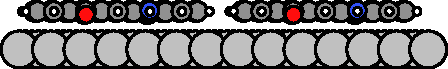
\includegraphics[width=\textwidth]{images/Models/qa_alpha-2_long-side.pdf}
    \caption{Long side view of the revised structure model for the $\alpha$-phase of \ac{QA} on the Ag(100) surface.}
    \label{fig:qa_alpha_long_side}
\end{figure}

The long side view of the structure model for the $\alpha$-phase of \ac{QA} on the Ag(100) surface in \autoref{fig:qa_alpha_long_side} shows the adsorption height of the \ac{QA} molecule, which is based on the results of the \ac{NIXSW} measurements. It shows that the \ac{QA} molecule is adsorbed face-on on the Ag(100) surface, with the O atoms of the carbonyl groups pointing towards the surface. The other atoms of the \ac{QA} molecule are more or less at the same height, and only exhibit minor differences in the adsorption height.

The different heights of the O and N atoms, which are the atoms that are involved in the hydrogen bonds, is clearly visible in the long side view. The H atom, that is part of the amine group and thus forms a hydrogen bond with the keto group of a neighboring molecule, is expected to be located at a height between the heights of the N and O atoms. However, the adsorption height of the H atoms are not known.

The long side view also shows the distance between two 1D chains of \ac{QA} molecules, which is described by the unit cell vector $\mathbf{b}_2$. As there are no hydrogen bonds between the 1D chains, the distance between the chains is larger than the distance between the molecules within the chains, which is described by the unit cell vector $\mathbf{b}_1$. The distance between the molecules withing the chains is visible in the short side view of the structure model for the $\alpha$-phase of \ac{QA} on the Ag(100) surface in \autoref{fig:qa_alpha_short_side}.

\begin{figure}[htbp]
    \centering
    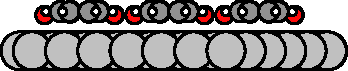
\includegraphics[width=\textwidth]{images/Models/qa_alpha-2_short-side.pdf}
    \caption{Short side view of the revised structure model for the $\alpha$-phase of \ac{QA} on the Ag(100) surface.}
    \label{fig:qa_alpha_short_side}
\end{figure}

Furthermore, the short side view of the structure model for the $\alpha$-phase of \ac{QA} on the Ag(100) surface in \autoref{fig:qa_alpha_short_side} shows the approach of the O atoms of the carbonyl groups towards the surface. The O atoms are closer to the surface than the other atoms of the \ac{QA} molecule. This view also shows that the O atoms are located outside of the ring, allowing them to be more flexible in their adsorption height and thus to interact more strongly with the surface. The N atoms of the amine groups, on the other hand, are located within the ring and thus are more constrained in their adsorption height.


%%%%%%%%%%%%%%%%%%%%%%%%%%%%%%%%%%%%%%%%%%%%%%%%
\newpage
\section{Structure model for the \texorpdfstring{$\beta$}{beta}-phase}

In contrast to the structure model for the $\alpha$-phase of \ac{QA} on the Ag(100) surface, the structure model for the $\beta$-phase significantly differs from the literature, which is shown in \autoref{fig:literature_beta}. 


\begin{figure}[htbp]
    \centering
    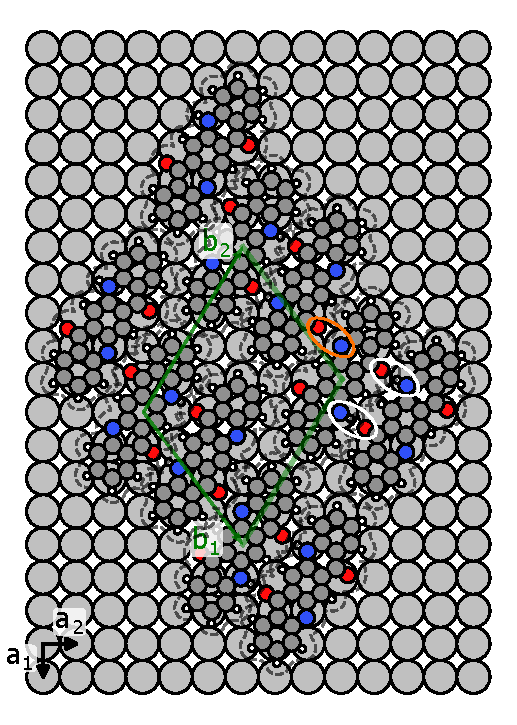
\includegraphics[width=0.92\textwidth]{images/Models/qa_beta-2_top-view_with_vdw-hbonds.pdf}
    \caption{Top view of the structure model for the $\beta$-phase of \ac{QA} on the Ag(100) surface. The hydrogen bonds between the O1 and N1 components are marked with white ellipses, while the missing hydrogen bond due to deprotonation between the O2 and N2 component is marked with an orange ellipse. The van der Waals radii of the atoms are shown as dashed grey lines. The unit cell is indicated by the green rectangle with the corresponding unit cell vectors $\mathbf{b}_1$ and $\mathbf{b}_2$ and is based on reference \cite{Humberg2020}.}
    \label{fig:qa_beta_top_view}
\end{figure}

As already observed in the literature\autocite{Humberg2020}, the $\beta$-phase of \ac{QA} on the Ag(100) surface is not homochiral, but consists of dimers with opposite chirality. In between the \ac{QA} molecules in the dimers, there are 2 hydrogen bonds. The hydrogen bonds are formed between the O1 and N1 components of the neighboring molecules. These two hydrogen bonds are shown in \autoref{fig:qa_beta_top_view} as white ellipses.

However, between the different dimers, there are no hydrogen bonds at all. This is in contrast to the previous structure model from the literature, which is shown in \autoref{fig:literature_beta}, where it was assumed that there is one hydrogen bonds between the neighboring molecules in different dimers. The missing hydrogen bond between the neighboring molecules in different dimers is indicated by the orange ellipse in \autoref{fig:qa_beta_top_view}.

As the \ac{XPS} measurements have shown, the N2 component is deprotonated in the $\beta$-phase and is thus not able to form a hydrogen bond with the O2 component of a neighboring molecule. As the number of the N atoms in the N1 and N2 component are the same, there are only two hydrogen bonds per molecule to its two neighbors in the $\beta$-phase, which are formed between the O1 and N1 components of neighboring molecules in the dimers.

Furthermore, the $\beta$-phase exhibits a commensurate strucure, which is described by the unit cell vectors $\mathbf{b}_1$ and $\mathbf{b}_2$ in \autoref{fig:qa_beta_top_view}. The unit cell and its structure is based on reference \cite{Humberg2020}. This shows that the \ac{QA} molecules in the $\beta$-phase are adsorbed at specific adsorption sites on the Ag(100) surface, which is in contrast to the $\alpha$-phase, where the molecules are adsorbed in a \ac{pol} structure. 

The atom that is most likely adsorbed at a specific adsorption site is the deprotonated N2 component, which is not involved in any hydrogen bonds and located very close to the surface. The N2 component is thus expected to be adsorbed at a specific adsorption site on the Ag(100) surface, which is most likely a on-top site, as almost all N atoms of the N2 component are located above the Ag atoms in the structure model in \autoref{fig:qa_beta_top_view}.

Nevertheless, some of the N atoms of the N atoms are not located above the Ag atoms. This could be due to the fact that the unit cell of the $\beta$-phase is very large and contains two \ac{QA} molecules and 27 Ag atoms per unit cell. Thus, it is possible that the positions of the N atoms are not perfectly accurate in the structure model in \autoref{fig:qa_beta_top_view}, which is based on \ac{LEED} and \ac{STM} measurements from the literature.\autocite{Humberg2020} In addition, the bonds in the \ac{QA} molecule are not perfectly rigid, and thus the positions of the atoms could be slightly different from the positions in the structure model.

Another interesting aspect of the structure model for the $\beta$-phase of \ac{QA} on the Ag(100) surface is the shift between the different dimers along the unit cell vector $\mathbf{b}_2$. This shift can be seen in the long side view of the structure model in \autoref{fig:qa_beta_long_side}, where the \ac{QA} molecule at the back is shifted to the right compared to the dimer at the front.

\begin{figure}[htbp]
    \centering
    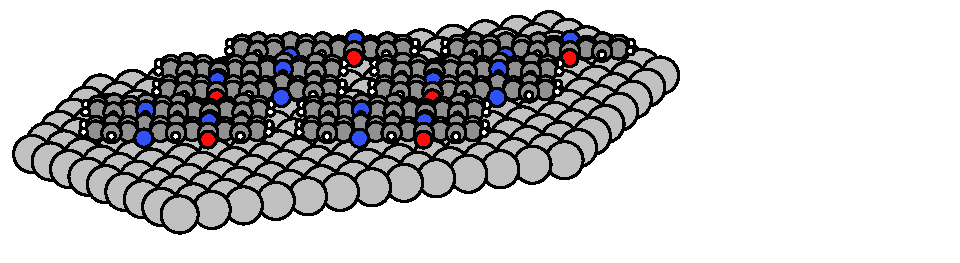
\includegraphics[width=\textwidth]{images/Models/qa_beta_long-side-slightly-up-2.pdf}
    \caption{Long side view of the revised structure model for the $\beta$-phase of \ac{QA} on the Ag(100) surface. The underlying Ag atoms at the corners of \autoref{fig:qa_beta_top_view} are deleted for better visibility.}
    \label{fig:qa_beta_long_side}
\end{figure}

As already observed for the $\alpha$-phase, the \ac{QA} molecules in the $\beta$-phase form molecular chains in one direction, which is described by the unit cell vector $\mathbf{b}_1$. The distance between the different molecular chains are described by the unit cell vector $\mathbf{b}_2$ and are clearly visible in \autoref{fig:qa_beta_long_side}.

Furthermore, this view already indicates the different adsorption heights of the different atoms in the \ac{QA} molecule in the $\beta$-phase, which are based on the results of the \ac{NIXSW} measurements. The N2 component is the closest atom to the surface. For a more detailed view of the different adsorption heights, the long side view of only one \ac{QA} molecule is shown in \autoref{fig:qa_beta_long_side_1} from both sides of the molecule.

\begin{figure}[htbp]
    \centering
    \subfloat[Deprotonated N2 atom]{%
        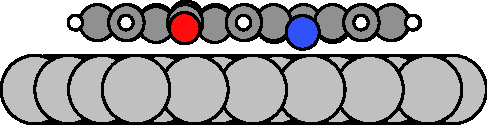
\includegraphics[width=0.48\textwidth]{images/Models/qa_beta_long-side-3-1.pdf}
    }
    \hfill
    \subfloat[Protonated N1 atom]{%
        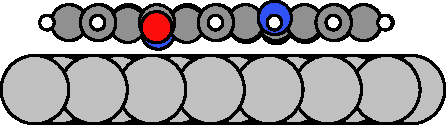
\includegraphics[width=0.48\textwidth]{images/Models/qa_beta_long-side-3-2.pdf}
    }
    \caption{Long side views of the revised structure model for the $\beta$-phase of \ac{QA} on the Ag(100) surface. The left image shows the side of the deprotonated N2 component, while the right image shows the side of the N1 component.}
    \label{fig:qa_beta_long_side_1}
\end{figure}

\autoref{fig:qa_beta_long_side_1} shows the different adsorption heights of the different atoms in the \ac{QA} molecule in the $\beta$-phase. The deprotonated N2 component is the closest atom to the surface, while the protonated N1 component is the highest atom, which is even higher than the C atoms. The O atoms are located closer to the surface than the C atoms, but are not as close to the surface as the N2 component. Furthermore, the different C atoms have different adsorption heights as well, which can be seen at the $\mathrm{C_{CO}}$ and $\mathrm{C_{O}}$ components, that are closer to the surface than the other C atoms and thus have an adsorption height between the other C atoms and the O atoms. The different adsorption heights can be explained by the different interactions of the atoms with the surface, which was done in detail in \autoref{sec:NIXSW-beta}.

This behavior of the different adsorption heights of the different atoms in the \ac{QA} molecule can also be seen in the short side view of the structure model for the $\beta$-phase on the Ag(100) surface in \autoref{fig:qa_beta_short_side}.

\begin{figure}[htbp]
    \centering
    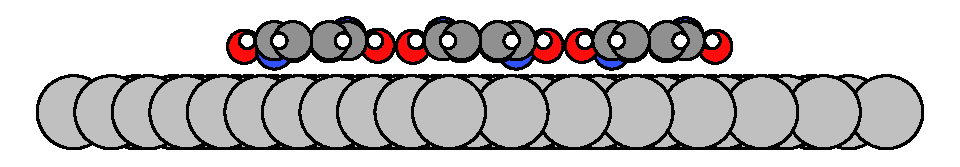
\includegraphics[width=\textwidth]{images/Models/qa_beta_short-side.pdf}
    \caption{Short side view of the revised structure model for the $\beta$-phase of \ac{QA} on the Ag(100) surface. The two \ac{QA} molecules on the left are one dimer and form two hydrogen bonds, while the \ac{QA} molecule on the right is part of the neighboring dimer without hydrogen bonds to the shown \ac{QA} molecule.}
    \label{fig:qa_beta_short_side}
\end{figure}

Again, it is visible that the O atoms are closer to the surface than the C atoms, while the N2 component is the closest atom to the surface and the N2 component is the highest atom. This view enable a more detailed view at atoms involved in the hydrogen bonds, as the hydrogen bonds are perpendicular to the view. The hydrogen bonds are formed between the left and the middle \ac{QA} molecule, which are part of the same dimer.

The N1 component is the located higher than the O1 component. However, the difference is only about 0.1~\si{\angstrom}. The small difference in the height can be compensated by the H atom of the amine group, which is expected to be located at a height between the N1 and O1 component.

\cleardoublepage